\documentclass[12pt,letterpaper]{article}
%\documentstyle[11pt]{article}
\usepackage[utf8]{inputenc}
\usepackage{amsmath}
\usepackage{xfrac}
\usepackage{amsfonts}
\usepackage{amssymb}
\usepackage[version = 3]{mhchem}
\usepackage{chemstyle}
%%For Table perhaps%%
%\usepackage{graphics}
\usepackage{graphicx}
\usepackage{epstopdf}
\usepackage{tabularx,ragged2e,booktabs,caption}
\newcolumntype{C}[1]{>{\Centering}m{#1}}
\renewcommand\tabularxcolumn[1]{C{#1}}
\usepackage[left=1cm,right=1cm,top=1cm,bottom=1cm]{geometry}
\usepackage{subcaption} 
\usepackage{caption}
\usepackage[colorlinks]{hyperref}
\usepackage[svgnames]{xcolor}
\hypersetup{citecolor=DeepPink4}
\hypersetup{linkcolor=DarkRed}
\hypersetup{urlcolor=DarkBlue}
\usepackage{cleveref}
\usepackage{enumerate}

\begin{document}
\setlength{\parindent}{0cm} 


\frenchspacing


\title {\Large{\textbf{Problem Set 9 ---Key}}\\ \large{CENG 340--Introduction to Environmental Engineering\\
Instructor: Deborah Sills\\ \textbf{November 20, 2013}}}

\author {}
\date {}
\maketitle

\vspace{-1in}

 


\begin{enumerate}


\item \emph{(12.5 pts)} \textbf{\large{Monod Kinetics}}\\
A kinetic study of the bacterial utilization of methanol was conducted and yielded the following data:\\

\begin{minipage}{\linewidth}
\centering
\begin{tabular}{|c|c|}\toprule[1.25pt]
\bf Substrate, S (mg/L)	& \bf dS/dt ($\mathrm{\frac{mg}{L\times hr}}$)	\\\midrule
2	& 1\\ \hline\
4	& 1.5\\ \hline\
6	& 1.8\\ \hline\
8	& 2\\ \hline\
10 & 2.14\\
\bottomrule[1.25pt]

\end {tabular}\par
\end{minipage}\\

S = concentration of methanol.\\

In addition, biomass concentration (bacterial concentration, X) was maintained at a constant 100 mg/L during the study. 

\begin{enumerate}

\item From this data, determine the parameters for a Monod substrate utilization model, presented below.

\begin{align}
\mathrm{-\frac{dS}{dt} = \frac{\mu_{max}XS}{K_s + S}}
\end{align}

The model was fit to Eq.1 using Kaleidagraph's non-linear curve fitting package.  The data and model fit are presented in Figure 1.

\begin{figure}
\centering
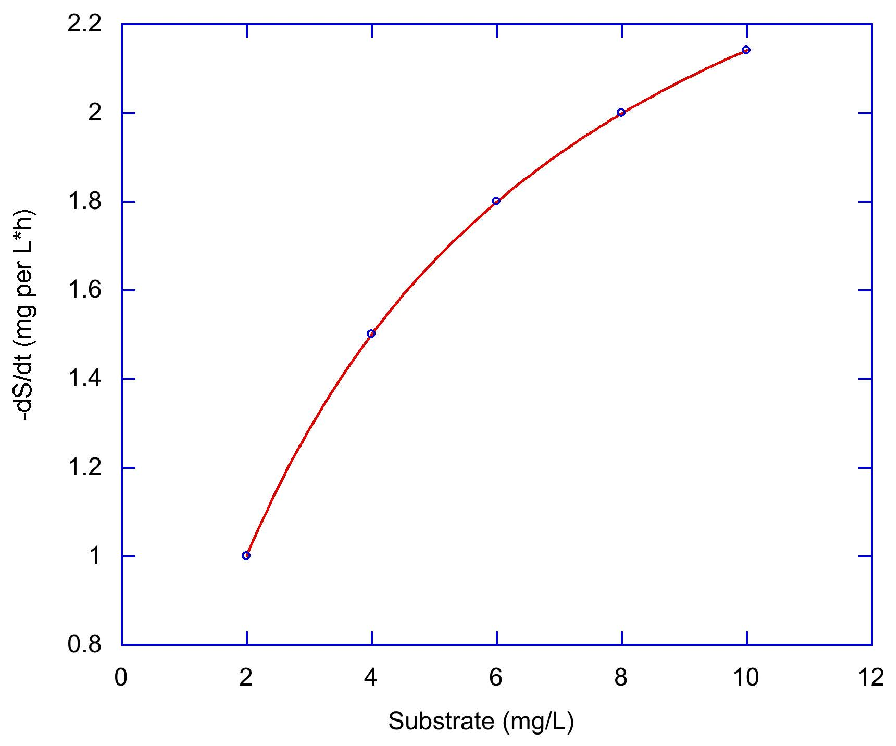
\includegraphics[width=0.4\textwidth]{PS9_monod}\caption{Growth rate of microroganisms as a function of substrate concentration. Circles represent data and the line represents a model fit.}
\end{figure}
\pagebreak

The fitted parameters are as follows:

$\mu_{max}$ = 0.03 $\mathrm{\frac{mg\, S}{mg\, X\times h}}$ = 0.72 $\mathrm{\frac{mg\, S}{mg\, X\times day}}$\\

$\mathrm{K_s}$ = 4 mg/L


\item This model can be used to predict the concentration of methanol in a well-mixed pond that has an indigenous bacteria population close to that used in the kinetic study above.The concentration of the bacteria in the pond is, however, 10\% of that of the kinetic study, and this bacterial concentration is relatively constant in the pond.  Determine the methanol concentration in the pond 5 days after the pond was contaminated with 200 mg/L of methanol. Assume the pond behaves as a batch reactor (no inflow/outflow) and that no methanol escapes by evaporation. Hint: employ the ``diphasic'' or ``mixed-order'' Monod model.\\

Since S is much bigger than K$_s$, Eq. 1 simplifies to a zero-order equation presented as Eq. 2:

\begin{align}
\mathrm{-\frac{dS}{dt} = \mu_{max}X}
\end{align}

Eq. 2 can be integrated, resulting in Eq. 3: 

\begin{align}
\mathrm{-(S(t) - S(0)) = \mu_{max}Xt}
\end{align}

Eq. 3 can be rearranged resulting in Eq. 4:

\begin{align}
\mathrm{S(t) = S(0) - \mu_{max}Xt}
\end{align}

Inputting numbers results in:

\begin{align*}
\mathrm{S(5) = 200\, \frac{mg}{L} - 0.72\, \frac{mg\, S}{mg\, X\times day}\times 10\, \frac{mg\, X}{L} \times 5\, day}
\end{align*}

S = 164 mg/L, which is still much bigger (at least one order of magnitude bigger) than K$_s$.  In other words, the zero-order equation is still valid.


\begin{align*}
\mathrm{S = \frac{K_s(1 + k_d\theta_c)}{\theta_c(\mu_{max} - k_d) - 1}}
\end{align*}

\begin{align*}
\mathrm{\theta_{c(min)} = \frac{1}{\mu_{max} - k_d}}
\end{align*}



\end{enumerate}




\end{enumerate}
\end{document}